\documentclass[crop,dvipsnames,tikz]{standalone}

\usetikzlibrary{calc}

\begin{document}
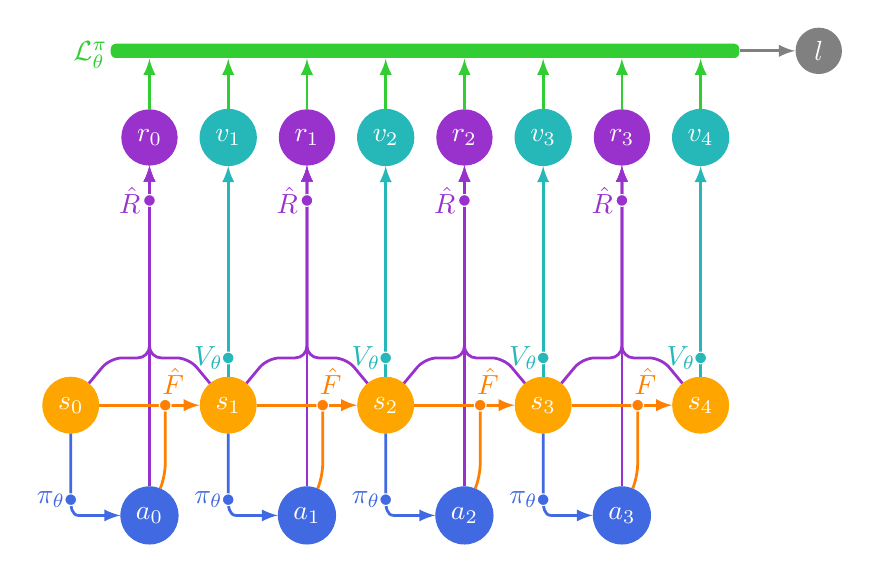
\begin{tikzpicture}

    \def\nodes{3}
    \def\nnodes{4}
    
    % Loop to place numbers
    \foreach \i in {0,...,\nodes} {
        \pgfmathsetmacro{\sx}{\i*2}
        \pgfmathsetmacro{\ax}{\i*2+1}
        
        % Draw number
        \node[circle, fill=Orange,draw=Orange] (s\i) at (\sx, 0) {\color{white}$s_\i$};
        \node[circle, fill=RoyalBlue,draw=RoyalBlue] (a\i) at (\ax, -1.4) {\color{white}$a_\i$};
        \node[circle, fill=DarkOrchid,draw=DarkOrchid] (r\i) at (\ax, +3.4) {\color{white}$r_\i$};

    }
    \pgfmathsetmacro{\sx}{\nnodes*2}
    \node[circle, draw=Orange, fill=Orange] (s\nnodes) at (\sx, 0) {\color{white}$s_\nnodes$};


    % reward function
    \foreach \i in {0, ..., \nodes} {
        \pgfmathtruncatemacro{\j}{\i+1}
        \draw[-latex,line width=1,color=DarkOrchid] (a\i) -- (r\i);
        \draw[-latex,line width=1,color=DarkOrchid,rounded corners=1ex] (s\i) -- ($(s\i) + (+.5,.6)$) -- ($(a\i) + (0,2)$) -- (r\i);
        \draw[-latex,line width=1,color=DarkOrchid,rounded corners=1ex] (s\j) -- ($(s\j) + (-.5,.6)$) -- ($(a\i) + (0,2)$) -- (r\i);
        \node[circle, fill=DarkOrchid,draw=white, inner sep=1.5pt] (tmp) at ($(r\i) - (0,.8)$) {};
        \node at ($(tmp) - (.25,0)$) {\color{DarkOrchid}$\hat{R}$};
    }

    % policy function
    \foreach \i in {0, ..., \nodes} {
        \draw[-latex,line width=1,color=RoyalBlue] (s\i) -- ($(s\i) - (0,1.2)$) to[out=270,in=180] ($(a\i) - (.9,0)$) -- (a\i);
        \node[circle, fill=RoyalBlue,draw=white, inner sep=1.5pt] (tmp) at ($(s\i) - (0,1.2)$) {};
        \node at ($(tmp) - (.25,0)$) {\color{RoyalBlue}$\pi_\theta$};
    }

    % value function
    \foreach \i in {1, ..., \nnodes} {
        \node[circle, fill=BlueGreen,draw=BlueGreen] (v\i) at ($(s\i) + (0,3.4)$) {\color{white}$v_\i$};
        \draw[-latex,line width=1, color=BlueGreen] (s\i) --  (v\i);
        \node[circle, fill=BlueGreen,draw=white, inner sep=1.5pt] (tmp) at ($(s\i) + (0,.6)$) {};
        \node at ($(tmp) - (.25,0)$) {\color{BlueGreen}$V_\theta$};
    }

    % transition function
    \foreach \i in {0, ..., \nodes} {
        \pgfmathtruncatemacro{\j}{\i+1}
        \draw[-latex,line width=1, color=orange] (s\i) -- (s\j) ;
        \draw[-, line width=1, color=orange, rounded corners=1ex] (a\i) -- ($(a\i) + (.2,.5)$) -- ($(s\j) - (.8,0)$); 
        \node[circle, fill=orange,draw=white, inner sep=1.5pt] (tmp) at ($(s\j) - (.8,0)$) {};
        \node at ($(tmp) + (.1,.3)$) {\color{orange}$\hat{F}$};
    }

    % loss policy function
    \draw[draw=white,fill=LimeGreen,rounded corners=.5ex] ($(r0) + (-.5, 1)$) rectangle ($(v4) + (.5,1.2)$); 
    \node at ($(r0) + (-.75,1.05)$) {\color{LimeGreen}$\mathcal{L}^\pi_\theta$};
    \foreach \i in {0, ..., \nodes} {
        \pgfmathtruncatemacro{\j}{\i+1}
        \draw[-latex,line width=1, color=LimeGreen] (r\i) -- ($(r\i) + (0,1)$);
        \draw[-latex,line width=1, color=LimeGreen] (v\j) -- ($(v\j) + (0,1)$);
    }

    \node[circle, fill=gray] (l) at ($(v\nnodes) + (1.5,1.1)$) {\color{white}$l$};
    \draw[-latex,line width=1, color=gray] ($(v\nnodes) + (.5,1.1)$) -- (l);




\end{tikzpicture}
\end{document}

